\problemname{ASDFGH}

Bjarki var að taka þátt í forritunarkeppni um daginn, en þá mætti allt í einu
Ágúst illkvittni tvíburi hans á svæðið og fór að fikta með lyklaborðið hans
Bjarka. Hann renndi fingrinum sínum fram og til baka yfir lyklaborðið þannig að
á skjáinn komu langar runur af stöfum sem eru á sömu röð á lyklaborðinu. Bjarki
byrjaði að reyna að hreinsa út þær línur sem Ágúst hafði skrifað inn, en hann
hafði skrifað inn alltof margar línur! Hjálpiði Bjarka að finna út hvaða línur eru hvað!

\begin{figure}
    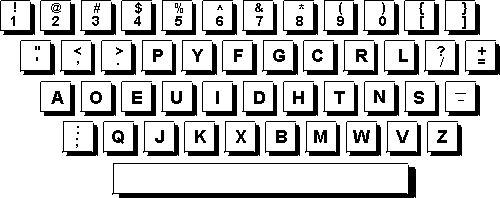
\includegraphics{dvorak.png}
\end{figure}

\section*{Inntak}
Inntakið samanstendur af einni línu með einn streng sem inniheldur enska lágstafi.

\section*{Úttak}
Skrifið út ``Jebb'' ef að strengurinn samastendur af stöfum sem eru á sömu
línunni á Dvorak lyklaborði, annars ``Neibb''.
